\label{chpt:results:evolutionary modelling} % for referencing this chapter elsewhere, use \ref{chpt:label}
\lhead{\emph{Inferring mass loss rate from donor properties}} % This is for the header on each page - perhaps a shortened title

\section{Reproducing the canonical CV donor tracks}
\label{sect:results:reproducing K11 tracks}

First, I demonstrate that MESA can closely reproduce the two \citet{knigge11} donor tracks -- recall from \S\ref{sect:introduction:the missing aml problem} that two such tracks are constructed, a `standard' track with only typical gravitational braking below the period gap, and an `optimal' track that amplifies gravitational braking by $2.47\times$.
By default, MESA shuts off magnetic braking when the donor becomes fully convective, a practice which I motivate in \S\ref{sect:introduction:the missing aml problem} to be spurious. Instead, MESA is altered for a fixed magnetic braking cutoff at $0.2 M_\odot$, arbitrarily fixing the donor mass of the period gap in line with \citet{knigge11}.
In addition, \citet{Pala2017a} added a subroutine to MESA that allows for the amplification of gravitational braking below the period gap. This was used to reproduce the `optimal' track. Note that the donor physics was configured as described in \S\ref{sect:modelling:MESA configs}, and the model is initialised with some additional binary configuration:
\begin{itemize}
    \item The two objects begin as $M_{\rm donor} = 0.65 M_\odot$, $M_{\rm wd} = 0.82$, at an orbital period of 12 hours.
    \item The white dwarf is not allowed to retain any accreted material,
    \begin{itemize}
        \item \lstinline{mass_transfer_beta = 1.0}, \lstinline{limit_retention_by_mdot_edd = .false.}
    \end{itemize}
    \item The white dwarf is considered as a point mass, with no evolution over time,
    \begin{itemize}
        \item \lstinline{evolve_both_stars = .false.}
    \end{itemize}
\end{itemize}

These changes are enough to reproduce the \citet{knigge11} tracks to a reasonable degree; Figure~\ref{fig:results:MESA can reproduce the K11 tracks} shows the four model tracks in the short period regime.
Note that the small humps at $\sim 0.13 M_\odot$ in the MESA models are due to MESA switching do a different equation of state, and is expected.
The small difference in gradient between the MESA models and the \citet{knigge11} models is due to the donor having a differing mass-radius relationship, as this model does not yet include the star spot physics described in \S\ref{sect:modelling:starspots in MESA} for reasons given in the next section.
With a more tailored donor configuration this could likely be improved without introducing the star spot physics at all, but this is not the focus of this study and the agreement is considered acceptable even with the suboptimal settings.

\begin{figure}
    \centering
    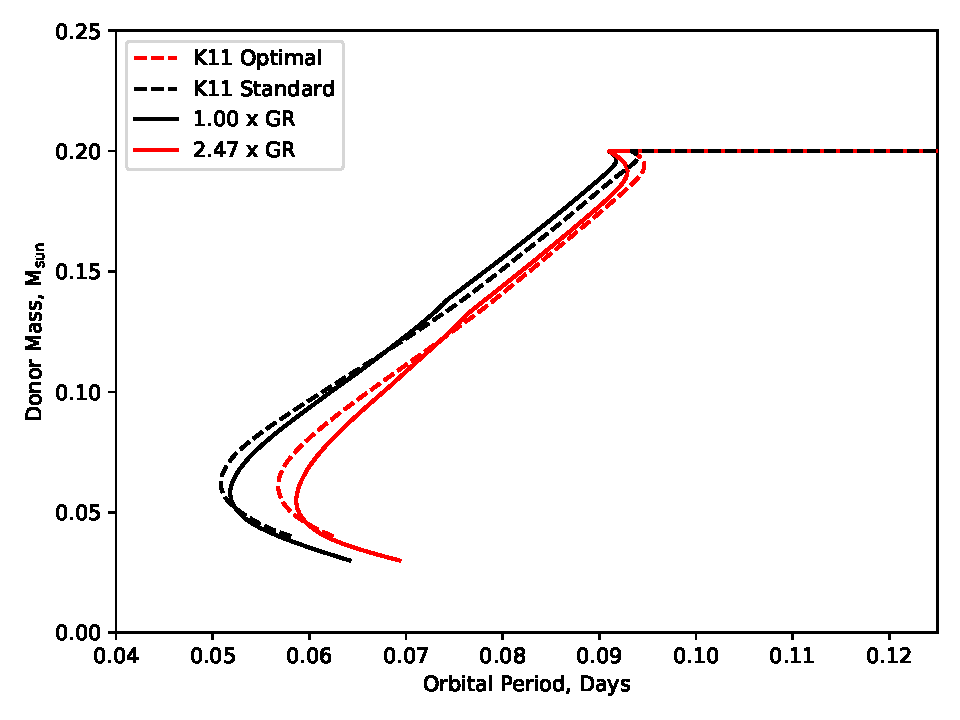
\includegraphics[width=.9\textwidth]{figures/modelling/reproducing_K11_tracks_fspot0.000.pdf}
    \caption{Showing how well MESA can reproduce the canonical \citet{knigge11} donor tracks. {\bf Solid lines} are MESA tracks, and {\bf dotted lines} are the \citet{knigge11} tracks. {\bf Black} lines have only gravitational braking below the period gap, and {\bf red} lines gave gravitational braking at $2.47\times$ strength.}
    \label{fig:results:MESA can reproduce the K11 tracks}
\end{figure}



\section{For what range of masses can we extract mass loss rates?}
\label{sect:results:MESA massloss allowable mass range}

This section evaluates the feasibility of using the radius of a star to extract present-day mass loss rates.
The analysis of this section does not include any star spots, i.e. $f_{\rm spot} = 0$ for these models.

Recall from \S\ref{sect:introduction:period minimum and bouncers} the two timescales that govern the response of the donor to mass loss: $\tau_{\rm KH}$ and $\tau_{\dot M}$. These timescales are calculated by
\begin{align}
    \tau_{\rm KH} \propto& \frac{M_{\rm donor}^2}{L_{\rm donor} R_{\rm donor}} \\[8pt]
    \tau_{\dot M} =& \frac{\dot M}{M_{\rm donor}}
\end{align}

If $\tau_{\rm KH} \ll \tau_{\dot M}$, the donor is able to maintain thermal equilibrium and is indistinguishable from a singleton star of the same mass.
If $\tau_{\rm KH} \gg \tau_{\dot M}$, the donor is \textit{not} able to maintain equilibrium, and mass loss is fast and adiabatic. The donor is inflated by mass loss, but because the star cannot adjust on thermal timescales, the degree of inflation becomes sensitive to the mass loss \textit{history} of the donor.
However, calculating the two timescales for CVs reveals that $\tau_{\rm KH} \sim \tau_{\dot M}$ \citep{knigge11} - meaning that most CV donors are \textit{almost} able to maintain thermal equilibrium, but are still mildly affected by mass loss.
Under this almost-equilibrium regime, mass loss induces some degree of radius inflation in the donor, but because the star still adjusts on thermal timescales, the degree of inflation only depends on the present-day average $\dot M$. In this regime, we can discard the mass loss history of the donor, and use the radius inflation as a diagnostic for the baseline mass loss rate.
This is also the justification for the CV tracks in \S\ref{sect:results:reproducing K11 tracks} to not include the star spot radius correction. As the donor decreases in mass, the necessary spot parameters to correct its radius will change (refer to \S\ref{sect:modelling:tuning star spots to observations}). However, the donor structure would only react to a change in spot parameters on the $\tau_{\rm KH}$ timescale, causing a CV donor model to effectively have the `wrong' spot parameters for its mass, due to the time lag between parameters changing and the donor radius responding to that change.


Whether a donor radius is sensitive to its $\dot M$ history can be considered as a function of $M_{\rm donor}$. As $M_{\rm donor}$ falls, $\tau_{\rm KH}$ begins to rise faster than $\tau_{\dot M}$; Figure~\ref{fig:results:how does tauKH and tauMdot vary with donor mass} shows this trend, produced by a MESA model of a CV using the configuration provided in \citet{Paxton_2015}.
The rise in $\tau_{\rm KH}$ relative to $\tau_{\dot M}$ becomes significant at $\sim 0.1 M_\odot$, around the mass the donor enters the fast, adiabatic $\tau_{\rm KH} \gg \tau_{\dot M}$ period bouncer phase c.f.~\S\ref{sect:introduction:period minimum and bouncers}.
\begin{figure}
    \centering
    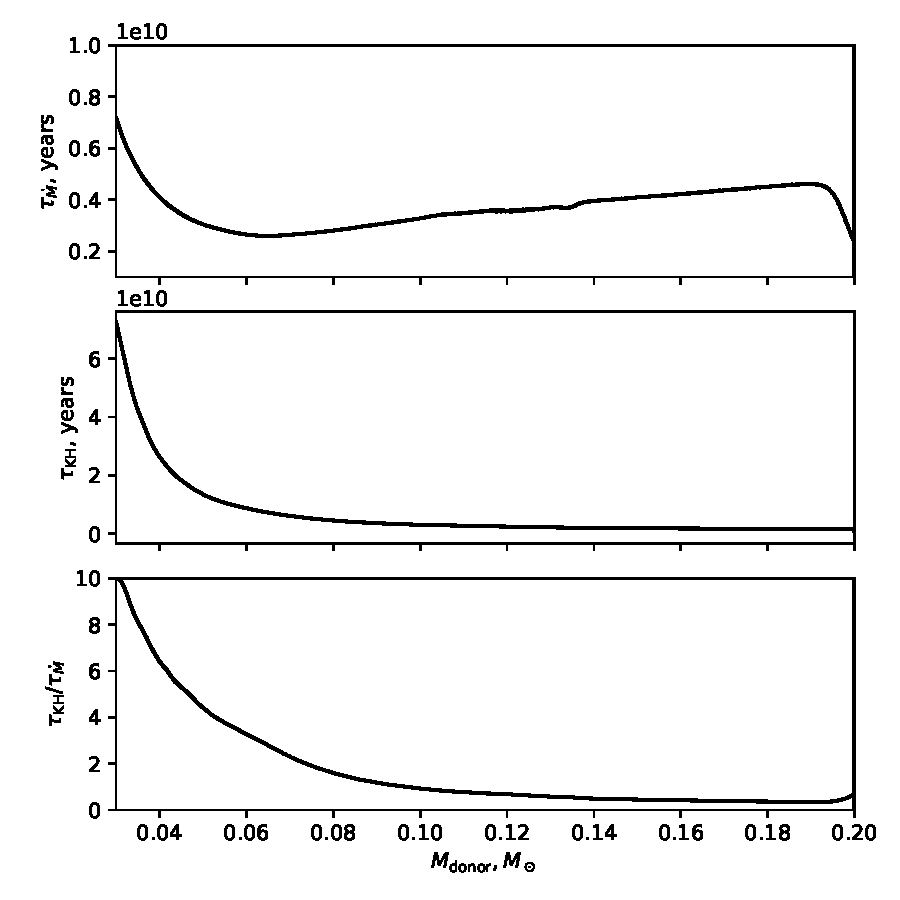
\includegraphics[width=\textwidth]{figures/modelling/tau_both_vs_donor_mass_AML000.pdf}
    \caption{Showing how the two timescales, $\tau_{\rm KH}$ and $\tau_{\dot M}$ vary with donor mass below the period gap in CV donors, as modelled by MESA \citep{Paxton_2015,Pala2017a}.}
    \label{fig:results:how does tauKH and tauMdot vary with donor mass}
\end{figure}

We can determine the range of donor masses for which $\tau_{\rm KH} \sim \tau_{\dot M}$ from MESA models.
First, a series of singleton models (using the MESA configuration given in \S\ref{sect:modelling:MESA configs}) were evaluated with varying amounts of fixed mass loss rates, uniformly spaced between $\log (\dot M, M_\odot \mathrm{yr}^{-1}) = -9.9 \rightarrow -10.8$.
Then, a series of MESA CV models were run with gravitational losses amplified by $x = 1 \rightarrow 6$, using the configuration and AML amplification in \S\ref{sect:results:reproducing K11 tracks}.
Finally, each model has its radius, $R$, and $\dot M$ extracted at $0.1 M_\odot$. Since the CV models have varying $\dot M$ and the singleton models do not, if $\dot M$ history does not affect radius inflation the radii between the two sets of models will match, and a disagreement indicates that history plays a significant role in radius inflation.
 Figure~\ref{fig:results:comparing radii at 0.1Msun} shows this, and little divergence between the two sets of radii is visible. However, note that higher $\dot M$ do show a small degree of divergence.
\begin{figure}
    \centering
    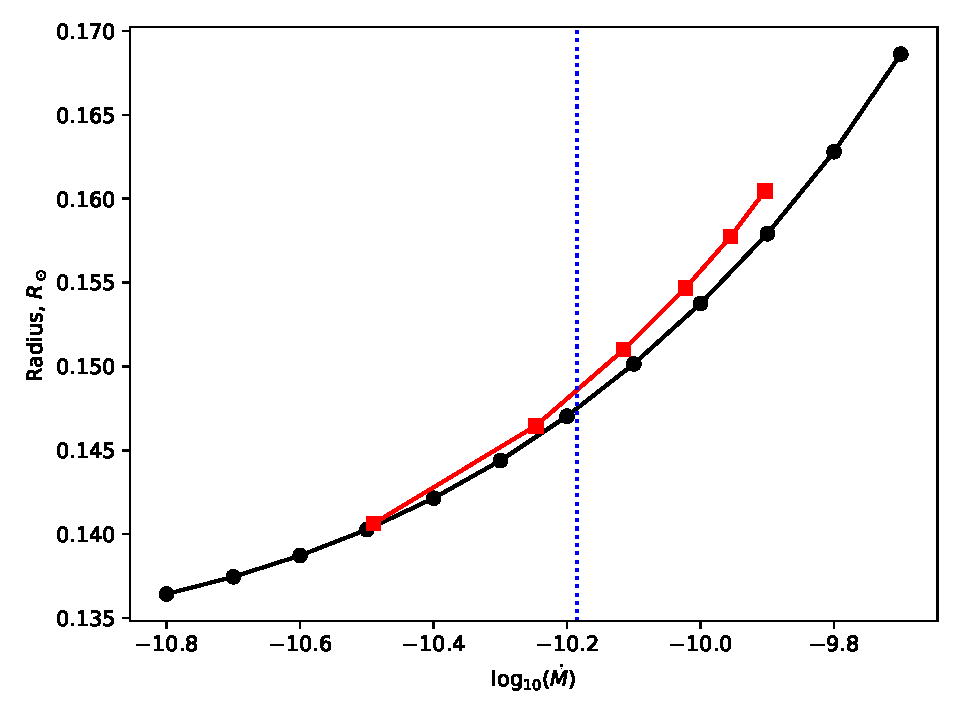
\includegraphics[width=.8\textwidth]{figures/modelling/compare_0.1Msun_with_CV_track_K11_fig1.pdf}
    \caption{Showing the radius and mass loss extracted from MESA models at $0.1 M_\odot$. The {\bf black} line is a series of singleton models with constant mass loss, and the {\bf red} line is a series of CV models with gravitational AML amplified by $x = 1 \rightarrow 6$, with the lowest $\dot M$ on the left. The {\bf blue dotted line} shows $\dot M$ for a CV with $2.47\times$ gravitational braking strength as predicted by a MESA CV model.}
    \label{fig:results:comparing radii at 0.1Msun}
\end{figure}

By plotting the difference between the two sets of models, and repeating the same process for a range of masses, Figure~\ref{fig:results:comparing radii over a range of masses} is produced. Now, by looking at what level of divergence historical changes in $\dot M$ induces at various donor masses, we can evaluate what mass range is acceptable. The upper limit on mass must be $0.2 M_\odot$, as this is the enforced mass of the period gap, and for a lower limit I impose an acceptable level of disagreement of $3\%$. It can be seen that the minimum acceptable mass is then $0.08 M_\odot$.
\begin{figure}
    \centering
    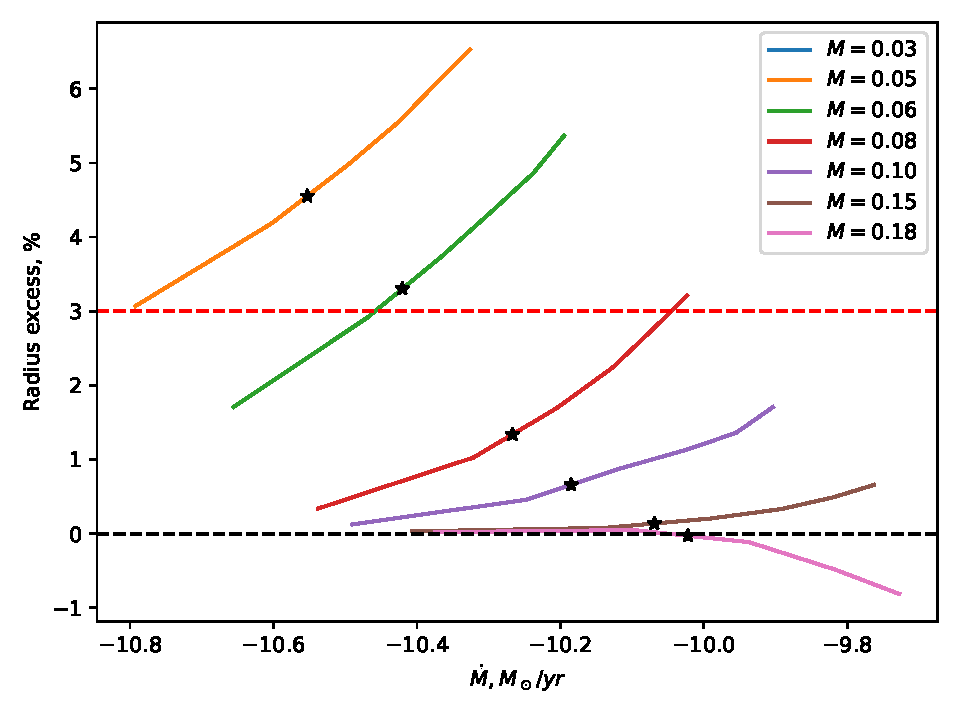
\includegraphics[width=\textwidth]{figures/modelling/compare_multiple_mass_with_CV_K11_fig1a.pdf}
    \caption{The inflation of CV model radii, $R_{CV}$ (whose $\dot M$ is time-dependent), over singleton model radii, $R_S$ (whose $\dot M$ is constant), from Figure~\ref{fig:results:comparing radii at 0.1Msun}, for a range of masses. The {\bf stars} on each line show the $\dot M$ and inflation for a model with gravitational braking at $2.47\times$ strength, mirroring the \citet{knigge11} optimal track. The {\bf red dashed line} shows the upper limit for acceptable disagreement, and the {\bf black dashed line} shows perfect agreement.}
    \label{fig:results:comparing radii over a range of masses}
\end{figure}



\section{Tuning star spot parameters to observations}
\label{sect:modelling:tuning star spots to observations}

With star spots implemented in MESA, the Brown relation can now be reproduced.
$x_{\rm spot}$ is fixed at 0 and $f_{\rm spot}$ is varied.
Since radius then increases monotonically with $f_{\rm spot}$, a binary chop is performed, optimising for $\Delta R = R_{\rm MESA} - (1.045\times R_{\rm Brown}) = 0$ at a stellar age of 2~Gyrs for a range of masses. The 4.5\% radius increase is to compensate for the non-spherical Roche geometry of the donor.
The resulting M-$f_{\rm spot}$ relation is shown in Figure~\ref{fig:modelling:fspot mass relationship}.

Below masses of $\sim 0.13 M_\odot$, the required $f_{\rm spot}$ becomes slightly negative, i.e. default MESA models are larger than observations plus the $4.5\%$ non-spherical correction.
Since a negative coverage fraction is unphysical, negative values of $f_{\rm spot}$ are set equal to 0, and it should be emphasised that derived mass loss rates become more unreliable below this mass.
However, the severity of this unreliability is not catastrophic, as the minimum value of $f_{\rm spot}$ is still reasonably close to 0.

There is significant scatter in the Brown mass-radius relation, that is not captured in these models. The inherent scatter in radius for the observations is $\sim 3\%$ between 0.1 and 0.2 $M_\odot$, which adds to the uncertainty in modelled radius inflation, and thus mass loss rate.
Whilst this may skew an individual system, on average the inferred mass loss from model radius should be accurate. Therefore, this effect should not skew the $\dot M$ results with a large enough sample size.

\begin{figure}
    \centering
    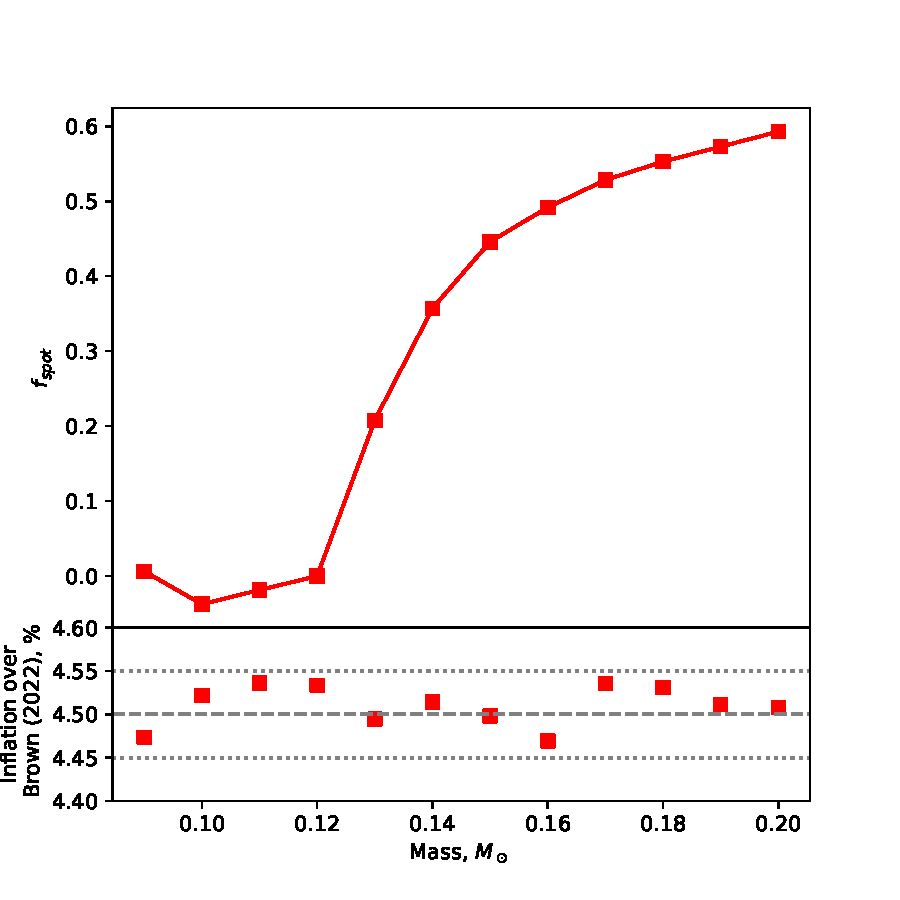
\includegraphics[width=\textwidth]{figures/modelling/fspot_relation_to_match_brown_plus_4.5.pdf}
    \caption{{\it Top}: The required $f_{\rm spot}$ that is applied to tune M dwarf MESA models to match the Brown relation, plus an added $4.5\%$ inflation due to non-spherical Roche geometry. {\it Bottom}: the residuals from the best fit value of $f_{\rm spot}$. Note that when finding the necessary value of $f_{\rm spot}$ to match the Brown relation $x_{\rm spot} \equiv 0$, and negative values of $f_{\rm spot}$ were allowed. However, in all subsequent modelling, negative $f_{\rm spot}$ were set to 0. {\bf Red squares} show evaluated MESA models.}
    \label{fig:modelling:fspot mass relationship}
\end{figure}



\section{Inferred mass loss rates of CV donors}
\label{sect:modelling:donor mass loss rates}

Overall, there are 30 systems with eclipse-modelled characterisations available for use.
However, not all are suitable; as shown in \S\ref{sect:results:MESA massloss allowable mass range}, the donor mass range for which modelling is possible is $0.08 M_\odot < M_{\rm donor} < 0.20 M_\odot$.
Applying this cut to the data leaves 22 systems, 12 from \citet{McAllister2019} and 10 from this thesis.
SDSS J1524 is included despite having a donor mass below the lower limit of $0.08 M_\odot$, as the measurement is within $1\sigma$ of this limit.
The properties of these donors, and their inferred $\dot M$, is given in Table~\ref{table:results:mdot modelling}.

The reported central values were optimised with a binary chop algorithm, but uncertainties were characterised by interpolation. This is considered a valid uncertainty, as the interpolation produced a central value within $1\sigma$ of the binary chop value in all cases.
Note that there was a single exception to this; in the case of ASASN-17fo, whilst the interpolator was unable to find an appropriate $\dot M$, the binary chop approach converged on a reasonable value of $\log (\dot M,\ M_{\odot}\ {\rm yr}^{-1} = -10.86$. This leaves this value with no characterised error, so an arbitrary error of $\pm 0.5$ dex was used during later analysis.
Note that not all systems in Table~\ref{table:results:mdot modelling} are assigned a $\dot M$.
This is due some donors being smaller than the Brown relation adjusted for non-spherical geometry, resulting in negative inflation that cannot be achieved by the introduction of mass loss.

Table~\ref{table:results:Jdot results} shows the AML rates calculated using Equation~\ref{eqn:modelling:Jdot from Mdot} for the systems for which $\dot M$ could be calculated from donor properties. Also shown is the ratio between the observed AML, and the AML predicted by the `standard' MESA donor track for a CV donor of the same mass.

\begin{table*}
    \centering
    \caption{The inferred $\dot M$ for eclipse-modelled CVs. For the Source column, `W20' are from Chapter~\ref{chpt:results:three peculiar white dwarfs}, `W22' are from Chapter~\ref{chpt:results:characterisation of 12 new CVs}, `M19' are systems modelled by \citet{McAllister2019}, `M17a' is from \citet{mcallister2017}, `M17b' is from \citet{mcallister2017b}, `M15' is from \citet{mcallister2015}, `S11' are from \citet{Savoury2011}, and `C10' is from \citet{copperwheat2010}.}
    \label{table:results:mdot modelling}
    \begin{tabular}{llccc}
        \hline \\
        {\bf System Name:} & \textbf{Source} & \textbf{$M_{\rm donor}, M_\odot$}  & \textbf{$R_{\rm donor}, R_\odot$}  & \textbf{$\log_{10}(\dot M,\ M_\odot / {\rm yr})$} \\
        \hline \hline \\
        ASASSN-14hq      & W22  &  $0.097 \pm 0.002$    & $0.157 \pm 0.001$     & $  -9.89 \pm 0.01$    \\
        ASASSN-15pb      & W22  &  $0.148 \pm 0.008$    & $0.209 \pm 0.004$     & $  -9.99 \pm 0.43$    \\
        ASASSN-17fo      & W22  &  $0.109 \pm 0.002$    & $0.1436 \pm 0.0007$   & $ -10.86$             \\
        AY For           & W22  &  $0.106 \pm 0.006$    & $0.162 \pm 0.003$     & $  -9.91 \pm 0.51$    \\
        CSS090419        & W22  &  $0.087 \pm 0.012$    & $0.152 \pm 0.007$     & $  -9.85 \pm 0.16$    \\
        CSS090622        & W22  &  $0.105 \pm 0.010$    & $0.155 \pm 0.005$     & $ -10.04 \pm 0.77$    \\
        MAST0014         & W22  &  $0.123 \pm 0.006$    & $0.165 \pm 0.003$     & $ -10.27 \pm 0.58$    \\
        OGLE82           & W22  &  $0.132 \pm 0.004$    & $0.170 \pm 0.002$     & $ -11.68 \pm 0.54$    \\
        SDSS J0748       & W22  &  $0.085 \pm 0.010$    & $0.128 \pm 0.005$     & $ -10.43 \pm 0.28$    \\
        SDSS J1524       & W22  &  $0.074 \pm 0.008$    & $0.132 \pm 0.005$     & $ -10.11 \pm 0.17$    \\
        CSS080623        & M19  &  $0.081 \pm 0.005$    & $0.128 \pm 0.002$     & $ -10.34 \pm 0.13$    \\
        CSS110113        & M19  &  $0.105 \pm 0.007$    & $0.149 \pm 0.003$     & $ -10.27 \pm 0.73$    \\
        OY Car           & M19  &  $0.093 \pm 0.004$    & $0.139 \pm 0.002$     & $ -10.27 \pm 0.06$    \\
        SDSS 0901        & M19  &  $0.138 \pm 0.007$    & $0.182 \pm 0.003$     & $ -10.54 \pm 0.71$    \\
        SDSS 1152        & M19  &  $0.094 \pm 0.016$    & $0.147 \pm 0.006$     & $ -10.06 \pm 0.38$    \\
        SSS100615        & M19  &  $0.083 \pm 0.005$    & $0.128 \pm 0.003$     & $ -10.38 \pm 0.16$    \\
        CTCV J2354-4700  & S11  &  $0.101 \pm 0.003$    & $0.146 \pm 0.002$     & $ -10.24 \pm 0.01$    \\
        SDSS J1152+4049  & S11  &  $0.087 \pm 0.006$    & $0.142 \pm 0.003$     & $ -10.06 \pm 0.08$    \\
        OU Vir           & S11  &  $0.116 \pm 0.002$    & $0.164 \pm 0.001$     & $ -10.06 \pm 0.10$    \\
        XZ Eri           & S11  &  $0.091 \pm 0.004$    & $0.135 \pm 0.002$     & $ -10.35 \pm 0.08$    \\
        SDSS 0903        & S11  &  $0.099 \pm 0.004$    & $0.136 \pm 0.002$     & $ -10.67 \pm 0.07$    \\
        SDSS 1227        & S11  &  $0.088 \pm 0.003$    & $0.137 \pm 0.001$     & $ -10.24 \pm 0.05$    \\
        SDSS 1502        & S11  &  $0.0781 \pm 0.0008$  & $0.1241 \pm 0.0003$   & $ -10.37 \pm 0.04$    \\
        SDSS 1501        & S11  &  $0.077 \pm 0.010$    & $0.122 \pm 0.005$     & $ -10.42 \pm 0.38$    \\
        ASASSN-14ag      & M17b &  $0.093 \pm 0.013$    & $0.135 \pm 0.007$     & $ -10.41 \pm 0.27$    \\
        ASASSN-14kb      & W22  &  $0.134 \pm 0.004$    & $0.164 \pm 0.001$     & -                     \\
        CTCV 1300-3052   & M19  &  $0.166 \pm 0.006$    & $0.211 \pm 0.003$     & -                     \\
        DV UMa           & M19  &  $0.187 \pm 0.012$    & $0.215 \pm 0.005$     & -                     \\
        IY UMa           & M19  &  $0.141 \pm 0.007$    & $0.177 \pm 0.003$     & -                     \\
        SSS130413        & M19  &  $0.140 \pm 0.012$    & $0.163 \pm 0.004$     & -                     \\
        V713 Cep         & M19  &  $0.176 \pm 0.018$    & $0.208 \pm 0.005$     & -                     \\
        Z Cha            & M19  &  $0.152 \pm 0.005$    & $0.182 \pm 0.002$     & -                     \\
        CTCV J1300-3052  & S11  &  $0.177 \pm 0.021$    & $0.215 \pm 0.008$     & -                     \\
        DV UMa           & S11  &  $0.196 \pm 0.005$    & $0.218 \pm 0.002$     & -                     \\
        % ASASSN-16kr      & W20  &  $0.042 \pm 0.003$    & $0.106 \pm 0.003$     & $ -10.7 \pm 0.5$      \\
        % SSS111126        & W20  &  $0.0424 \pm 0.004$   & $0.107 \pm 0.003$     & $ -10.64 \pm 0.50$    \\
        % CSS090102        & W22  &  $0.059 \pm 0.003$    & $0.119 \pm 0.002$     & $ -10.25 \pm 0.50$    \\
        % SDSS 1501        & M19  &  $0.061 \pm 0.004$    & $0.113 \pm 0.003$     & $ -10.45 \pm 0.50$    \\
        % SDSS 1035        & S11  &  $0.048 \pm 0.001$    & $0.105 \pm 0.001$     & $ -10.74 \pm 0.50$    \\
        % PHL 1445         & M15  &  $0.064 \pm 0.005$    & $0.109 \pm 0.004$     & $ -10.66 \pm 0.50$    \\
        % SDSS J1057+2759  & M17a &  $0.044 \pm 0.002$    & $0.108 \pm 0.002$     & $ -10.51 \pm 0.50$    \\
        % ASASSN-17jf      & W20  &  $0.060 \pm 0.009$    & $0.112 \pm 0.005$     & -                     \\
        % GY Cnc           & M19  &  $0.394 \pm 0.022$    & $0.446 \pm 0.009$     & -                     \\
        % SDSS 1006        & M19  &  $0.37 \pm 0.06$      & $0.457 \pm 0.026$     & -                     \\
        % SDSS 1702        & S11  &  $0.223 \pm 0.010$    & $0.252 \pm 0.004$     & -                     \\
        % SDSS 1507        & S11  &  $0.058 \pm 0.002$    & $0.097 \pm 0.001$     & -                     \\
        % SDSS 1433        & S11  &  $0.0571 \pm 0.0007$  & $0.1074 \pm 0.0004$   & -                     \\
        % IP Peg           & C10  &  $0.55 \pm 0.02$      & $0.466 \pm 0.006$     & -                     \\
        \hline
    \end{tabular}
\end{table*}

\begin{table*}
    \centering
    \caption{The inferred AML rates for the CVs in this sample. $\dot J_{\rm total}$ is calculated from the inferred $\dot M$, and $\dot J_{\rm GR}$ is interpolated from the `standard' MESA track in Figure~\ref{fig:results:MESA can reproduce the K11 tracks}, at the relevant donor mass. Sources are keyed the same as Table~\ref{table:results:mdot modelling}.}
    \label{table:results:Jdot results}
    \begin{tabular}{llccc}
        \hline
        {\bf System Name:} & \textbf{Source}  & \textbf{$\log(\dot J_{\rm total})$} & \textbf{$\log(\dot J_{\rm GR})$} & \textbf{$\dot J_{\rm total} / \dot J_{\rm GR}$} \\
        \hline \hline
        ASASSN-16kr      &  W20                 & $26.49 \pm 0.48$                  & $26.06$                          &  $2.66$ \\
        SSS111126        &  W20                 & $26.45 \pm 0.51$                  & $26.08$                          &  $2.34$ \\
        ASASSN-14hq      &  W22                 & $27.16 \pm 0.02$                  & $26.68$                          &  $2.99$ \\
        ASASSN-15pb      &  W22                 & $27.09 \pm 0.42$                  & $26.80$                          &  $1.96$ \\
        ASASSN-17fo      &  W22                 & $26.24 \pm 0.50$                  & $26.71$                          &  $0.34$ \\
        AY For           &  W22                 & $27.18 \pm 0.50$                  & $26.71$                          &  $3.01$ \\
        CSS090102        &  W22                 & $26.77 \pm 0.51$                  & $26.43$                          &  $2.20$ \\
        CSS090419        &  W22                 & $27.16 \pm 0.16$                  & $26.65$                          &  $3.28$ \\
        CSS090622        &  W22                 & $27.00 \pm 0.77$                  & $26.70$                          &  $1.98$ \\
        MAS0014          &  W22                 & $26.84 \pm 0.61$                  & $26.75$                          &  $1.25$ \\
        OGLE82           &  W22                 & $25.42 \pm 0.52$                  & $26.77$                          &  $0.05$ \\
        SDSS J0748       &  W22                 & $26.64 \pm 0.28$                  & $26.64$                          &  $1.02$ \\
        SDSS J1524       &  W22                 & $26.99 \pm 0.18$                  & $26.58$                          &  $2.59$ \\
        CSS080623        &  M19                 & $26.71 \pm 0.14$                  & $26.62$                          &  $1.22$ \\
        CSS110113        &  M19                 & $26.90 \pm 0.72$                  & $26.70$                          &  $1.55$ \\
        OY Car           &  M19                 & $26.84 \pm 0.06$                  & $26.67$                          &  $1.50$ \\
        SDSS 0901        &  M19                 & $26.54 \pm 0.70$                  & $26.78$                          &  $0.57$ \\
        SDSS 1152        &  M19                 & $26.95 \pm 0.38$                  & $26.67$                          &  $1.92$ \\
        SDSS 1501        &  M19                 & $26.60 \pm 0.50$                  & $26.45$                          &  $1.40$ \\
        SSS100615        &  M19                 & $26.73 \pm 0.17$                  & $26.63$                          &  $1.27$ \\
        SDSS J1057+2759  &  M17a                & $26.60 \pm 0.52$                  & $26.11$                          &  $3.05$ \\
        ASASSN-14ag      &  M17b                & $26.59 \pm 0.28$                  & $26.67$                          &  $0.84$ \\
        PHL 1445         &  M15                 & $26.39 \pm 0.50$                  & $26.49$                          &  $0.79$ \\
        CTCV J2354-4700  &  S11                 & $26.90 \pm 0.02$                  & $26.69$                          &  $1.61$ \\
        SDSS J1152+4049  &  S11                 & $26.92 \pm 0.08$                  & $26.64$                          &  $1.87$ \\
        OU Vir           &  S11                 & $27.00 \pm 0.11$                  & $26.73$                          &  $1.83$ \\
        XZ Eri           &  S11                 & $26.67 \pm 0.08$                  & $26.66$                          &  $1.03$ \\
        SDSS 1035        &  S11                 & $26.37 \pm 0.53$                  & $26.21$                          &  $1.42$ \\
        SDSS 0903        &  S11                 & $26.43 \pm 0.07$                  & $26.69$                          &  $0.55$ \\
        SDSS 1227        &  S11                 & $26.85 \pm 0.06$                  & $26.65$                          &  $1.57$ \\
        SDSS 1502        &  S11                 & $26.67 \pm 0.05$                  & $26.60$                          &  $1.17$ \\
        SDSS 1501        &  S11                 & $26.64 \pm 0.39$                  & $26.60$                          &  $1.10$ \\
        % ASASSN-17jf      &  W20  & $      NaN \pm      NaN$ & $26.438957 \pm          NaN $ &  $     NaN$ \\
        % ASASSN-14kb      &  W22  & $      NaN \pm      NaN$ & $26.771382 \pm          NaN $ &  $     NaN$ \\
        % CTCV 1300-3052   &  M19  & $      NaN \pm      NaN$ & $26.821457 \pm          NaN $ &  $     NaN$ \\
        % DV UMa           &  M19  & $      NaN \pm      NaN$ & $26.847761 \pm          NaN $ &  $     NaN$ \\
        % GY Cnc           &  M19  & $      NaN \pm      NaN$ & $28.717578 \pm          NaN $ &  $     NaN$ \\
        % IY UMa           &  M19  & $      NaN \pm      NaN$ & $26.787612 \pm          NaN $ &  $     NaN$ \\
        % SDSS 1006        &  M19  & $      NaN \pm      NaN$ & $28.658590 \pm          NaN $ &  $     NaN$ \\
        % SSS130413        &  M19  & $      NaN \pm      NaN$ & $26.786238 \pm          NaN $ &  $     NaN$ \\
        % V713 Cep         &  M19  & $      NaN \pm      NaN$ & $26.834171 \pm          NaN $ &  $     NaN$ \\
        % Z Cha            &  M19  & $      NaN \pm      NaN$ & $26.802830 \pm          NaN $ &  $     NaN$ \\
        % CTCV J1300-3052  &  S11  & $      NaN \pm      NaN$ & $26.835421 \pm          NaN $ &  $     NaN$ \\
        % DV UMa           &  S11  & $      NaN \pm      NaN$ & $26.867454 \pm          NaN $ &  $     NaN$ \\
        % SDSS 1702        &  S11  & $      NaN \pm      NaN$ & $28.231211 \pm          NaN $ &  $     NaN$ \\
        % SDSS 1507        &  S11  & $      NaN \pm      NaN$ & $26.404859 \pm          NaN $ &  $     NaN$ \\
        % SDSS 1433        &  S11  & $      NaN \pm      NaN$ & $26.398756 \pm          NaN $ &  $     NaN$ \\
        % IP Peg           &  C10  & $      NaN \pm      NaN$ & $29.062496 \pm          NaN $ &  $     NaN$ \\
        \hline
    \end{tabular}
\end{table*}


\section{Mass loss from white dwarf effective temperatures}
\label{sect:modelling:white dwarf mass loss rates}

The characterised CVs also have the white dwarf temperature constrained to within $\sim 2000 \rm K$, allowing the short-term mass loss rate to also be inferred as suggested in \S\ref{sect:modelling:mdot from WD temperature}.
Note that, despite the large uncertainty in $T_{\rm eff}$, the errors are smaller than those obtained with the donor properties.
% Figure~\todo{Get this figure} compares the $\dot M$ found by each technique, plotted as a function of donor mass.

\begin{table}
    \centering
    \caption{The $\dot M$ found using the white dwarf properties for each system with a $\dot M$ measurement from donor properties. Sources are keyed the same as Table~\ref{table:results:mdot modelling}}
    \label{table:results:Mdot from white dwarf parameters}
    \begin{tabular}{llccc}
        \hline
        \textbf{Name} & \textbf{Source} & \textbf{$M_{\rm wd}, M_\odot$} & \textbf{$T_{\rm eff}$, K} & \textbf{$\log (\dot M, M_\odot {\rm yr}^{-1})$} \\
        \hline \hline \\
        ASASSN-14hq      &  W22  & $0.67 \pm 0.01$ & $14800\pm   800$ & $ -9.93 \pm 0.02$ \\
        ASASSN-14kb      &  W22  & $0.74 \pm 0.02$ & $17700\pm  1000$ & $ -9.90 \pm 0.03$ \\
        ASASSN-15pb      &  W22  & $0.72 \pm 0.03$ & $19200\pm  1600$ & $ -9.85 \pm 0.04$ \\
        ASASSN-17fo      &  W22  & $0.85 \pm 0.01$ & $14800\pm   600$ & $-10.03 \pm 0.02$ \\
        AY For           &  W22  & $0.78 \pm 0.02$ & $18200\pm   500$ & $ -9.91 \pm 0.02$ \\
        CSS090102        &  W22  & $0.62 \pm 0.03$ & $14800\pm  1200$ & $ -9.90 \pm 0.04$ \\
        CSS090419        &  W22  & $0.59 \pm 0.08$ & $18200\pm  9000$ & $ -9.79 \pm 0.28$ \\
        CSS090622        &  W22  & $0.67 \pm 0.06$ & $ 9800\pm  1500$ & $-10.11 \pm 0.08$ \\
        MAS0014          &  W22  & $0.86 \pm 0.03$ & $17300\pm  1000$ & $ -9.97 \pm 0.03$ \\
        OGLE82           &  W22  & $0.84 \pm 0.02$ & $18000\pm  4400$ & $ -9.95 \pm 0.12$ \\
        SDSS J0748       &  W22  & $0.80 \pm 0.05$ & $28400\pm  3300$ & $ -9.73 \pm 0.06$ \\
        SDSS J1524       &  W22  & $0.80 \pm 0.04$ & $12500\pm  1100$ & $-10.08 \pm 0.05$ \\
        ASASSN-16kr      &  W20  & $0.95 \pm 0.02$ & $11500\pm   300$ & $-10.19 \pm 0.01$ \\
        ASASSN-17jf      &  W20  & $0.70 \pm 0.03$ & $12020\pm   850$ & $-10.03 \pm 0.04$ \\
        SSS111126        &  W20  & $0.76 \pm 0.02$ & $22800\pm  1500$ & $ -9.80 \pm 0.03$ \\
        CSS080623        &  M19  & $0.71 \pm 0.02$ & $15500\pm  1700$ & $ -9.94 \pm 0.05$ \\
        CSS110113        &  M19  & $1.00 \pm 0.05$ & $14500\pm  2200$ & $-10.11 \pm 0.07$ \\
        CTCV 1300-3052   &  M19  & $0.72 \pm 0.02$ & $11000\pm  1000$ & $-10.09 \pm 0.04$ \\
        DV UMa           &  M19  & $1.09 \pm 0.03$ & $17400\pm  1900$ & $-10.07 \pm 0.05$ \\
        GY Cnc           &  M19  & $0.88 \pm 0.02$ & $25900\pm  2300$ & $ -9.81 \pm 0.04$ \\
        IY UMa           &  M19  & $0.96 \pm 0.01$ & $18000\pm  1000$ & $-10.00 \pm 0.02$ \\
        OY Car           &  M19  & $0.88 \pm 0.02$ & $18600\pm  2800$ & $ -9.95 \pm 0.07$ \\
        SDSS 0901        &  M19  & $0.75 \pm 0.02$ & $14900\pm  2000$ & $ -9.98 \pm 0.06$ \\
        SDSS 1006        &  M19  & $0.82 \pm 0.11$ & $16500\pm  2000$ & $ -9.97 \pm 0.08$ \\
        SDSS 1152        &  M19  & $0.62 \pm 0.04$ & $15900\pm  2000$ & $ -9.87 \pm 0.06$ \\
        SDSS 1501        &  M19  & $0.72 \pm 0.02$ & $14900\pm  1000$ & $ -9.96 \pm 0.03$ \\
        SSS100615        &  M19  & $0.88 \pm 0.03$ & $13600\pm  1500$ & $-10.09 \pm 0.05$ \\
        SSS130413        &  M19  & $0.84 \pm 0.03$ & $24000\pm  3000$ & $ -9.82 \pm 0.06$ \\
        V713 Cep         &  M19  & $0.70 \pm 0.02$ & $17000\pm  6000$ & $ -9.89 \pm 0.19$ \\
        Z Cha            &  M19  & $0.80 \pm 0.01$ & $16300\pm  1400$ & $ -9.97 \pm 0.04$ \\
        PHL 1445         &  M15  & $0.73 \pm 0.03$ & $13200\pm   700$ & $-10.02 \pm 0.03$ \\
        SDSS J1057+2759  &  M17a & $0.80 \pm 0.02$ & $13300\pm  1100$ & $-10.06 \pm 0.04$ \\
        ASASSN-14ag      &  M17b & $0.63 \pm 0.04$ & $14000\pm  2100$ & $ -9.93 \pm 0.07$ \\
        \hline
    \end{tabular}
\end{table}

\begin{table}
    \centering
    \caption{Table~\ref{table:results:Mdot from white dwarf parameters}, continued}
    \label{table:results:Mdot from white dwarf parameters cont}
    \begin{tabular}{llccc}
        \hline
        \textbf{Name} & \textbf{Source} & \textbf{$M_{\rm wd}, M_\odot$} & \textbf{$T_{\rm eff}$, K} & \textbf{$\log (\dot M, M_\odot {\rm yr}^{-1})$} \\
        \hline \hline \\
        CTCV J1300-3052  &  S11  & $0.74 \pm 0.01$ & $11100\pm   800$ & $-10.10 \pm 0.03$ \\
        CTCV J2354-4700  &  S11  & $0.94 \pm 0.03$ & $14800\pm   700$ & $-10.08 \pm 0.02$ \\
        SDSS J1152+4049  &  S11  & $0.56 \pm 0.03$ & $12400\pm  1400$ & $ -9.93 \pm 0.06$ \\
        OU Vir           &  S11  & $0.70 \pm 0.01$ & $22300\pm  2100$ & $ -9.77 \pm 0.04$ \\
        DV UMa           &  S11  & $1.10 \pm 0.02$ & $15500\pm  2400$ & $-10.13 \pm 0.07$ \\
        XZ Eri           &  S11  & $0.77 \pm 0.02$ & $15300\pm  1900$ & $ -9.98 \pm 0.06$ \\
        SDSS 1702        &  S11  & $0.91 \pm 0.03$ & $15200\pm  1200$ & $-10.05 \pm 0.04$ \\
        SDSS 1035        &  S11  & $0.84 \pm 0.01$ & $10000\pm  1100$ & $-10.20 \pm 0.05$ \\
        SDSS 1507        &  S11  & $0.89 \pm 0.01$ & $11300\pm  1000$ & $-10.17 \pm 0.04$ \\
        SDSS 0903        &  S11  & $0.87 \pm 0.01$ & $13300\pm  1700$ & $-10.09 \pm 0.06$ \\
        SDSS 1227        &  S11  & $0.80 \pm 0.02$ & $15900\pm  1400$ & $ -9.98 \pm 0.04$ \\
        SDSS 1433        &  S11  & $0.87 \pm 0.01$ & $12700\pm  1500$ & $-10.11 \pm 0.05$ \\
        SDSS 1502        &  S11  & $0.709\pm0.004$ & $11800\pm  1200$ & $-10.05 \pm 0.04$ \\
        SDSS 1501        &  S11  & $0.77 \pm 0.03$ & $10800\pm  1500$ & $-10.13 \pm 0.06$ \\
        IP Peg           &  C10  & $1.16 \pm 0.02$ & $12500\pm  2500$ & $-10.24 \pm 0.09$ \\

        \hline
    \end{tabular}
\end{table}